\documentclass{hcmutarticle}

\usepackage{amsmath}
\usepackage{multicol}
\setlength{\columnsep}{1cm}
% gói để tạo chữ giả, xóa đi khi viết báo cáo
%\usepackage{lipsum}

\usepackage{listings}
\usepackage{color}

\definecolor{dkgreen}{rgb}{0,0.6,0}
\definecolor{gray}{rgb}{0.5,0.5,0.5}
\definecolor{mauve}{rgb}{0.58,0,0.82}

\lstset{frame=tb,
	language=Java,
	aboveskip=3mm,
	belowskip=3mm,
	showstringspaces=false,
	columns=flexible,
	basicstyle={\small\ttfamily},
	numbers=none,
	numberstyle=\tiny\color{gray},
	keywordstyle=\color{blue},
	commentstyle=\color{dkgreen},
	stringstyle=\color{mauve},
	breaklines=true,
	breakatwhitespace=true,
	tabsize=3
}
% create the header for this file
\fancyhead[RO, LE]{\bf Bài toán khai báo tài liệu trích dẫn}


\begin{document}
\thispagestyle{empty}
\begin{center}
\LARGE\bfseries ĐẠI HỌC QUỐC GIA TP HỒ CHÍ MINH \\
TRƯỜNG ĐẠI HỌC BÁCH KHOA
\end{center}

\begin{center}

\includegraphics[scale=0.2]{hcmut.pdf}\\[1cm]
\end{center}

\vspace{1cm}

\begin{center}
\Large \bfseries BÁO CÁO BÀI TẬP LỚN MÔN NHẬN DIỆN MẪU VÀ HỌC MÁY\\[0.5cm]
\end{center}
\rule{\textwidth}{1pt}
\vspace{2pt}
\begin{center}
\Huge
\begin{tabular}{@{}l}
Study the PCA tool of WEKA \\
and apply it in feature extraction\\[6pt]
\end{tabular}
\end{center}
\rule{\textwidth}{1pt}\\[1cm]

\vspace{2cm}

\begin{minipage}[t]{0.60\linewidth}
\textbf{GVHD}: \\
\ PGS.TS. Dương Tuấn Anh
\end{minipage}
\begin{minipage}[t]{0.40\linewidth}
\textbf{Sinh viên thực hiện:}\\
Nguyễn Quốc Long - MSSV:1770023
\end{minipage}

\vspace{4cm}

\begin{center}

\textbf{TP.Hồ Chí Minh},
08/11/2018.

\end{center}



\newpage

\tableofcontents 

\newpage

\title{Bài luận tìm hiểu giải thuật Min-conficts}

\author{  Nguyễn Quốc Long\inst{1}} 

\institute{ MSSV: 1770023}




\maketitle



\begin{abstract}
Tài liệu tìm hiểu về giải thật PCA và phần mền WEKA.


\end{abstract}

\begin{keywords}
giảm chiều dữ liệu, giải thuật PCA, WEKA
\end{keywords} 


\section{Giới thiệu}

\textbf{Giảm chiều dữ liệu (Dimensionality Reduction)} 
 là một trong kỹ thuật quan trọng của Học Máy (Machine Learning). Các feature vectors trong các bài toán thực tế có thể có số chiều rất lớn, tới vài nghìn. Ngoài ra, số lượng các điểm dữ liệu cũng thường rất lớn. Nếu thực hiện lưu trữ và tính toán trực tiếp trên dữ liệu có số chiều cao này thì sẽ gặp khó khăn cả về việc lưu trữ và tốc độ tính toán. Vì vậy, giảm chiều dữ liệu sẽ làm tăng tốc độ tính toán nên đây là bước quan trọng trong nhiều bà toán học máy (đây cũng được gọi là phương pháp nén dữ liệu).
 
\textbf{Phân tích thành phần chính (Principal Component Analysis (PCA))}
 là một thuật toán Dimensionality Reduction dựa trên một mô hình tuyến tính. Phương pháp này dựa trên quan sát rằng dữ liệu thường không phân bố ngẫu nhiên trong không gian mà thường phân bố gần các đường/mặt đặc biệt nào đó. PCA xem xét một trường hợp đặc biệt khi các mặt đặc biệt có dạng tuyến tính là các không gian con (subspace).

\newpage

%%%%%%%%%%%%%%
\section{Giới thiệu công cụ Weka}\label{survey}
Weka (viết tắt của Waikato Environment for Knowledge Analysis) là một bộ phần mềm học máy được Đại học Waikato, New Zealand phát triển bằng Java. Weka là phần mềm tự do phát hành theo Giấy phép Công cộng GNU.

%%%%%%%%%%%%%%
\section{Giới thiệu phương pháp PCA}\label{dev}

PCA là một thủ tục toán học biến đổi một số thuộc tính tương quan thành một số lượng nhỏ hơn các thuộc tính không tương quan được gọi là các thành phần chính.

PCA là một phương pháp của Giảm chiều dữ liệu (Dimensionality reduction)

\textbf{Mục tiêu của PCA } là xác định cơ sở có ý nghĩa nhất để thể hiện lại một tập dữ liệu


Change of basis
- Is there another basis which is a liner combination of the original basis, that best re-express our data set


\begin{center}
	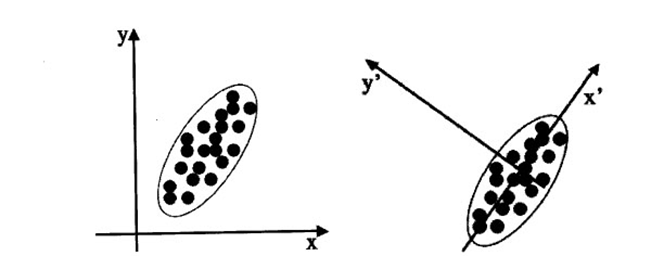
\includegraphics[scale=0.5]{image/figure.png}
	\text{Figure 2.7: Two different sets of coordinate axes.The second consists of a rotation and translation of the first and was found by using PCA.
	}
\end{center}
\section{Các bước rút trích dữ liệu đặc trưng bằng phương pháp PCA trong công cụ Weka}

\begin{multicols}{2}
	[
	Dữ liệu đầu vào cho chương trình WEKA
	]
	\begin{lstlisting}
	% 1. Title: PCA Database
	% 
	% 2. Sources:
	%      (a) Creator: nqlong
	%      (c) Date: Jan, 2019
	% 
	@RELATION iris
	
	@ATTRIBUTE x  NUMERIC
	@ATTRIBUTE y  NUMERIC
	@ATTRIBUTE class        {1,2}
	
	@data
	1,1,1
	1,2,1
	1,3,1
	2,1,1
	2,2,1
	2,3,1
	2,3.5,1
	2.5,2,1
	3.5,1,1
	3.5,2,1
	3.5,3,2
	3.5,4,2
	4.5,1,2
	4.5,2,2
	4.5,3,2
	5,4,2
	5,5,2
	6,3,2
	6,4,2
	6,5,2
	\end{lstlisting}
	
	\begin{center}
		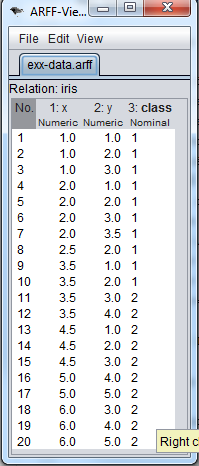
\includegraphics[scale=0.7]{image/data_weka.png}
	\end{center}
\end{multicols}

\[
\begin{bmatrix}
x_{11}       & x_{12} & x_{13} & \dots & x_{1n} \\
x_{21}       & x_{22} & x_{23} & \dots & x_{2n} \\
\hdotsfor{5} \\
x_{d1}       & x_{d2} & x_{d3} & \dots & x_{dn}
\end{bmatrix}
=
\begin{bmatrix}
x_{11} & x_{12} & x_{13} & \dots  & x_{1n} \\
x_{21} & x_{22} & x_{23} & \dots  & x_{2n} \\
\vdots & \vdots & \vdots & \ddots & \vdots \\
x_{d1} & x_{d2} & x_{d3} & \dots  & x_{dn}
\end{bmatrix}
\]

Tiếp theo, ta thiết lập cấu hình cho phần mềm WEKA
\begin{center}
	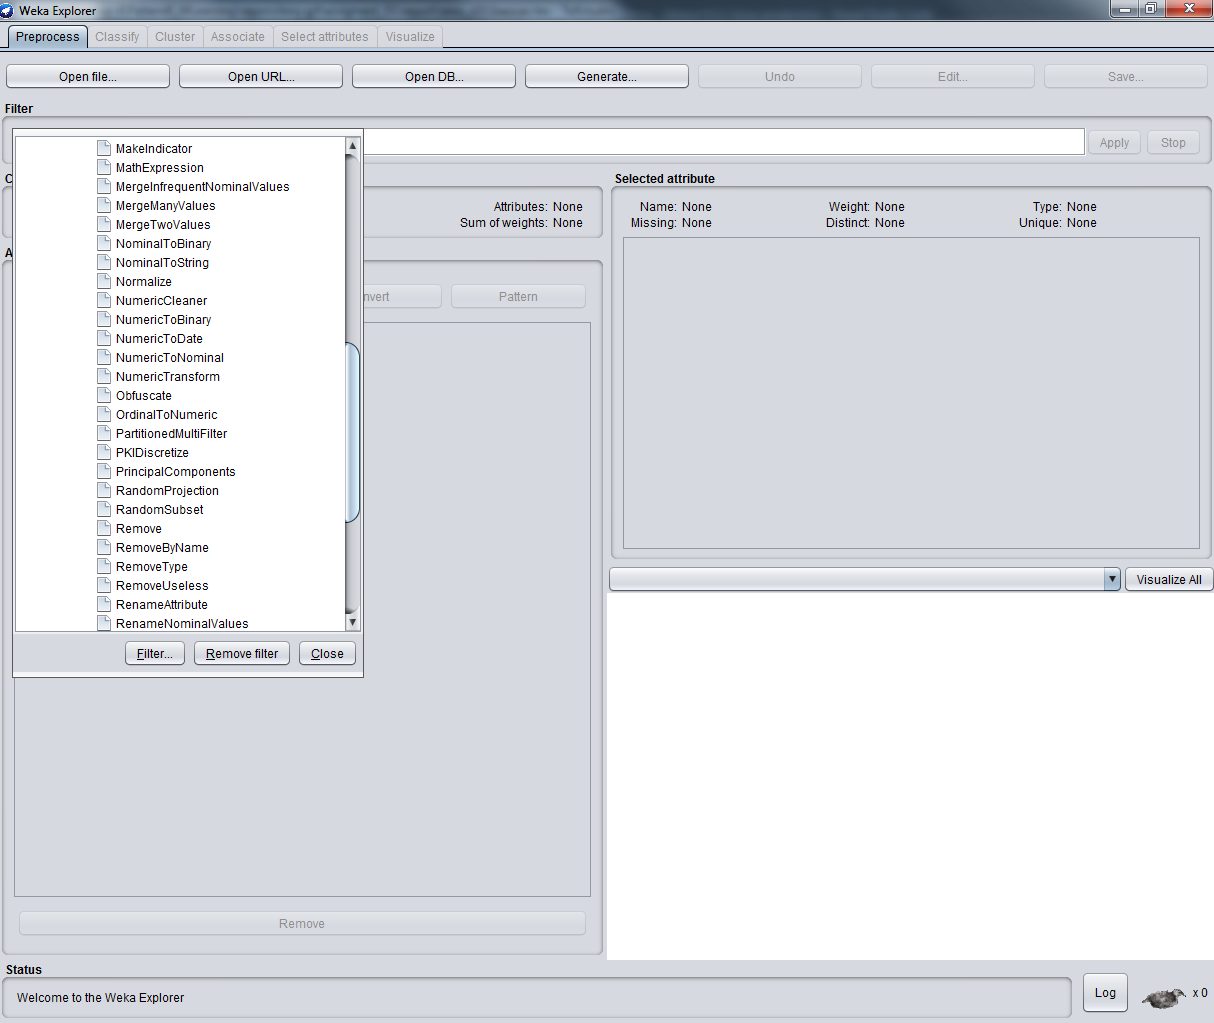
\includegraphics[scale=0.5]{image/step1.png}
\end{center}
% pca_1.png
% result_1.png

\begin{center}
	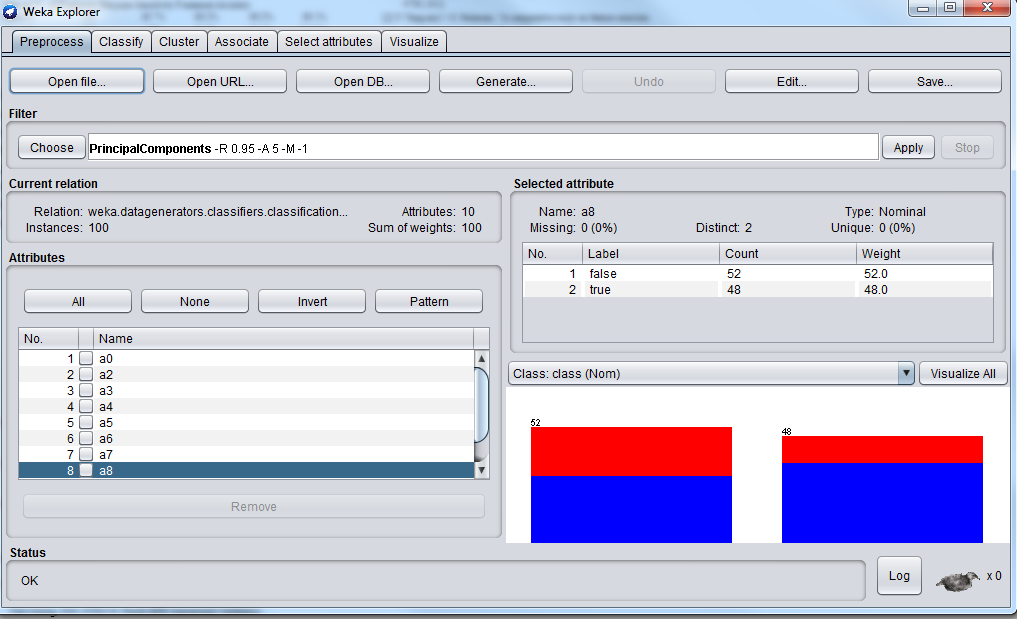
\includegraphics[scale=0.6]{image/pca_1.png}
\end{center}

\begin{center}
	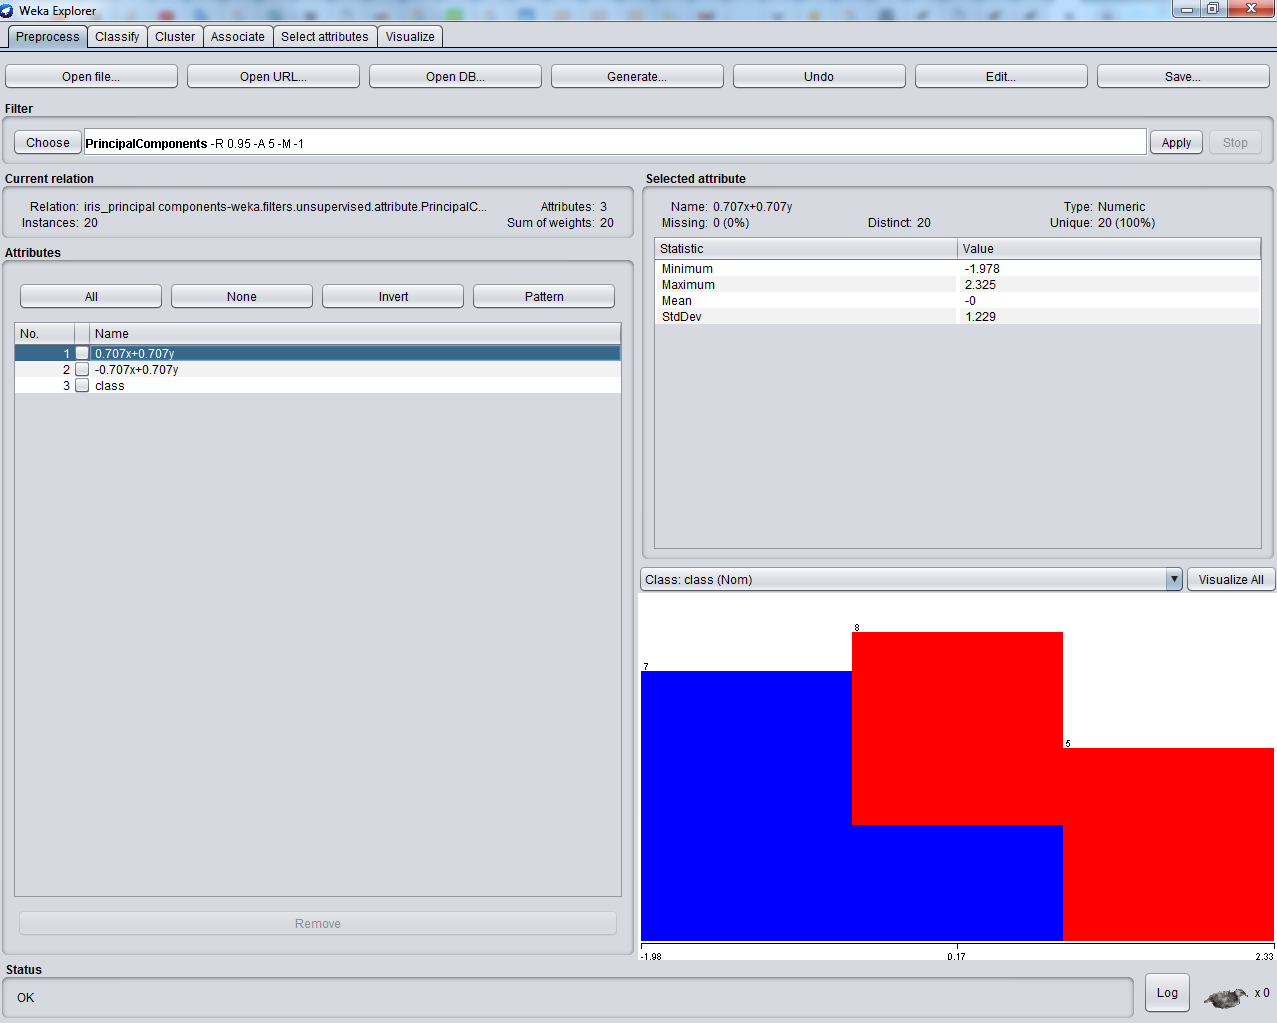
\includegraphics[scale=0.5]{image/result_1.png}
\end{center}

%%%%%%%%%%%%%%
\section{Kết Luận }\label{result}
Tài liệu được thực hiện  với sự giúp đỡ tận tình của giáo viên hướng dẫn, Thầy TS. Dương Tuấn Anh\\
Trong quá trình nghiên cứu, thực hiện không thể tránh khỏi những  thiếu sót, kính mong quý thầy  cô và các bạn đóng góp thêm để tài liệu thêm hoàn thiện.\\
Xin chân thành cảm ơn.


%%%%%%%%%%%%%%
\section{Tài liệu Tham Khảo }




%%%%%%%%%%%%%%%%%%%%%%%%%%%%%%%%%
%https://vi.wikipedia.org/wiki/Weka_(h%E1%BB%8Dc_m%C3%A1y)
http://en.wikipedia.org\\
https://machinelearningcoban.com/2017/06/15/pca/ \\
%https://waikato.github.io/weka-wiki/arff_stable/

%%%%%%%%%%%%%%

\end{document}



